\documentclass[12pt,oneside]{book}

\usepackage[a4paper,width=150mm,top=25mm,bottom=25mm]{geometry}
\usepackage[utf8]{inputenc}
\usepackage{amsmath}
\usepackage{amsthm}
\usepackage{amssymb}

\usepackage{tikz}
\usetikzlibrary{positioning,arrows}
\usetikzlibrary{decorations.pathmorphing}
\usetikzlibrary{decorations.markings}

\tikzset{
	fermion/.style={thick,draw=black, postaction={decorate}, decoration={markings,mark=at position 0.6 with {\arrow[black]{triangle 45}}}},
	photon/.style={decorate, draw=black, decoration={coil,aspect=0}},
	gluon/.style={decorate, draw=black, decoration={coil,amplitude=4pt, segment length=5pt}},
    higgs/.style={decorate, draw=black, dash pattern=on 3pt off 3pt},
}

\usepackage{fancyhdr}
\pagestyle{fancy}
	\renewcommand{\chaptermark}[1]{ \markboth{#1}{} }
	\renewcommand{\sectionmark}[1]{ \markright{#1}{} }
    \fancyfoot[C]{\thepage}

\setlength{\parindent}{0pt}

\begin{document}

\chapter*{Two higgs doublet model}

\section*{Introduction}

Two higgs doublets with two complex charged scalar fields $\phi^+_{i}$ and two neutral complex scalar fields $\phi^0_{i}$:

\begin{equation}
    \Phi_1 = \begin{pmatrix} \phi_1^{+} \\ \phi_1^{0} \end{pmatrix}, \quad \Phi_2 = \begin{pmatrix} \phi_2^{+} \\ \phi_2^{0} \end{pmatrix}
\end{equation}

Most general potential of a two higgs doublet model with the real constants $m_{11}^2, m_{22}^2, \lambda_1, \lambda_2, \lambda_3, \lambda_4$ and the complex constants $m_{12}^2, \lambda_5, \lambda_6, \lambda_7$:

\begin{align}
    V &= m_{11}^{2}\Phi_1^{\dagger}\Phi_1 + m_{22}^{2}\Phi_2^{\dagger}\Phi_2 - m_{12}^{2}\Phi_1^{\dagger}\Phi_2 - {m_{12}^2}^{\dagger}\Phi_2^{\dagger}\Phi_1 + \frac{\lambda_1}{2}(\Phi_1^{\dagger}\Phi_1)^2 + \frac{\lambda_2}{2}(\Phi_2^{\dagger}\Phi_2)^2 \\ \nonumber
    &+ \lambda_3(\Phi_1^{\dagger}\Phi_1)(\Phi_2^{\dagger}\Phi_2)^{2} + \lambda_4(\Phi_1^{\dagger}\Phi_2)(\Phi_2^{\dagger}\Phi_1)^{2} + \frac{\lambda_5}{2}(\Phi_1^{\dagger}\Phi_2)^2 + \frac{\lambda^{\dagger}_5}{2}(\Phi_2^{\dagger}\Phi_1)^2 \\ \nonumber
    &+ \lambda_6\Phi_1^{\dagger}\Phi_1\Phi_1^{\dagger}\Phi_2 + \lambda^{\dagger}_6\Phi_1^{\dagger}\Phi_1\Phi_2^{\dagger}\Phi_1 + \lambda_7\Phi_1^{\dagger}\Phi_2\Phi_2^{\dagger}\Phi_2 + \lambda^{\dagger}_7\Phi_1^{\dagger}\Phi_1\Phi_2^{\dagger}\Phi_1
\end{align} 

Minimum of the potential with $\sqrt{v_1^2 + v_2^2} = v$:

\begin{equation}
    \Phi_{1, \text{min}} = \begin{pmatrix} 0 \\ \frac{v_1}{\sqrt{2}}e^{i\varphi_1} \end{pmatrix}, \quad \Phi_{2, \text{min}} = \begin{pmatrix} 0 \\ \frac{v_2}{\sqrt{2}}e^{i\varphi_2} \end{pmatrix}
\end{equation}

Express two higgs doublets around vacuum expectation value:

\begin{equation}
    \Phi_1 = \begin{pmatrix} \phi_1^{+} \\ \frac{1}{\sqrt{2}}(e^{i\varphi_1} + \eta_1 + i\xi_1) \end{pmatrix}, \quad \Phi_2 = \begin{pmatrix} \phi_2^{+} \\ \frac{1}{\sqrt{2}}(e^{i\varphi_2} + \eta_2 + i\xi_2) \end{pmatrix}
\end{equation}

First model simplification:

\begin{itemize}
    \item Discrete Symmetry $\mathbb{Z}_2$: $\Phi_1 \to -\Phi_1$ (Absence of flavor-changing neutral currents)

    \begin{itemize}
        \item[$\to$] $\lambda_6 = \lambda_7 = 0$
    \end{itemize}

    \item Vanishing complex phases $\varphi_i = 0$ in vacuum expectation value (CP conservation)

    \begin{itemize}
        \item[$\to$] $\lambda_5$ and $m_{12}^2$ are real numbers
    \end{itemize}
\end{itemize}

Simplified potential:

\begin{align}
    V &= m_{11}^{2}\Phi_1^{\dagger}\Phi_1 + m_{22}^{2}\Phi_2^{\dagger}\Phi_2 - m_{12}^{2}(\Phi_1^{\dagger}\Phi_2 + \Phi_2^{\dagger}\Phi_1) + \frac{\lambda_1}{2}(\Phi_1^{\dagger}\Phi_1)^2 + \frac{\lambda_2}{2}(\Phi_2^{\dagger}\Phi_2)^2 \\ \nonumber
    &+ \lambda_3(\Phi_1^{\dagger}\Phi_1)(\Phi_2^{\dagger}\Phi_2)^{2} + \lambda_4(\Phi_1^{\dagger}\Phi_2)(\Phi_2^{\dagger}\Phi_1)^{2} + \frac{\lambda_5}{2}[(\Phi_1^{\dagger}\Phi_2)^2 + (\Phi_2^{\dagger}\Phi_1)^2] \\ \nonumber
\end{align} 

Defining parameter:

\begin{equation}
    \tan(\beta) = \frac{v_2}{v_1}, \quad \lambda_{ijk} \equiv \lambda_{i} + \lambda_{j} + \lambda_{k}
\end{equation}

Insert two higgs doublet from equation 4 into the simplified potential 5 and sort for the mass terms:

\begin{align}
    \mathcal{L}_{\phi^{\pm} \text{ mass}} &= \frac{1}{2}\begin{pmatrix} \phi^{+}_1, & \phi^{+}_2 \end{pmatrix} \underbrace{\begin{pmatrix} 2m_{11}^2 + \lambda_1 v_1^2 + \lambda_3 v_2^2 & -2m_{12}^2 + \lambda_{45}v_1 v_2 \\ -2m_{12} + \lambda_{45}v_1v_2 & 2m_{22}^2 + \lambda_2 v_2^2 + \lambda_3 v_1^2 \end{pmatrix}}_{M_\phi} \begin{pmatrix} \phi^{-}_1 \\ \phi^{-}_2 \end{pmatrix} \\
    \mathcal{L}_{\eta \text{ mass}} &= \frac{1}{2}\begin{pmatrix} \eta_1, & \eta_2 \end{pmatrix} \underbrace{\begin{pmatrix} 2m_{11}^{2} + \frac{3}{2}\lambda_1v_1 + \frac{1}{2}\lambda_{345}v_2^2 & -m_{12}^2 + \lambda_{345}v_1v_2 \\ -m_{12}^2 + \lambda_{345}v_1v_2 & 2m_{22}^{2} + \frac{3}{2}\lambda_2v_2 + \frac{1}{2}\lambda_{345}v_1^2\end{pmatrix}}_{M_\eta} \begin{pmatrix} \eta_1 \\ \eta_2 \end{pmatrix} \nonumber \\
    \mathcal{L}_{\xi \text{ mass}} &= \frac{1}{2}\begin{pmatrix} \xi_1, & \xi_2 \end{pmatrix} \underbrace{\begin{pmatrix} 2m_{11}^{2} + \frac{1}{2} \lambda_1v_1^2 + \frac{1}{2}v_2^2(\lambda_{34} - \lambda_5) & -m_{12}^2 + \lambda_5v_1v_2 \\ -m_{12}^2 + \lambda_5v_1v_2 & 2m_{22}^{2} + \frac{1}{2} \lambda_2v_2^2 + \frac{1}{2}v_1^2(\lambda_{34} - \lambda_5) \end{pmatrix}}_{M_\xi} \begin{pmatrix} \xi_1 \\ \xi_2 \end{pmatrix} \nonumber
\end{align}

After diagonalization of the mass matrices with $R_{a}^T M_a R_a$ with $a \in (\phi, \eta, \xi)$, the five Higgs bosons $h, H, A, H^{\pm}$ and the three Goldstone bosons $G, G^{\pm}$ can be expressed in terms of the $\phi, \eta, \xi$ and $R_a$:

\begin{align}
    \begin{pmatrix} h \\ H \end{pmatrix} &=  R^{-1}_\eta \begin{pmatrix} \eta_1 \\ \eta_2 \end{pmatrix} =  \begin{pmatrix} \sin(\alpha) & - \cos(\alpha) \\ -\cos(\alpha) & -\sin(\alpha) \end{pmatrix} \begin{pmatrix} \eta_1 \\ \eta_2 \end{pmatrix} \\
    \begin{pmatrix} G \\ A \end{pmatrix} &=  R^{-1}_\xi \begin{pmatrix} \xi_1 \\ \xi_2 \end{pmatrix} =  \begin{pmatrix} \cos(\beta) & \sin(\beta) \\ \sin(\beta) & -\cos(\beta) \end{pmatrix} \begin{pmatrix} \xi_1 \\ \xi_2 \end{pmatrix} \nonumber \\
    \begin{pmatrix} G^{\pm} \\ H^{\pm} \end{pmatrix} &=  R^{-1}_\phi \begin{pmatrix} \phi_1^{\pm} \\ \phi_2^{\pm} \end{pmatrix} =  \begin{pmatrix} \cos(\beta) & - \sin(\beta) \\ \sin(\beta) & \cos(\beta) \end{pmatrix} \begin{pmatrix} \phi_1^{\pm} \\ \phi_2^{\pm} \end{pmatrix} \nonumber
\end{align}

The mass terms of each boson is:

\begin{align}
    m_G^2 &= m_{G^{\pm}}^2 = 0 \\
    m_h^2 &= \frac{\sin^2(\alpha - \beta)}{\cos(\beta)\sin(\beta)}m_{12}^2 + v^2(\lambda_1 \cos^2(\beta) \sin^2(\alpha) + \lambda_2 \sin^2(\beta) \cos^2(\alpha) - \frac{1}{2} \lambda_{345} \sin(2\beta) \sin(2\alpha) \nonumber \\
    m_H^2 &= \frac{\sin^2(\alpha - \beta)}{\cos(\beta)\sin(\beta)}m_{12}^2 + v^2(\lambda_1 \cos^2(\beta) \cos^2(\alpha) + \lambda_2 \sin^2(\beta) \sin^2(\alpha) + \frac{1}{2} \lambda_{345} \sin(2\beta) \sin(2\alpha) \nonumber \\
    m_A^2 &= \frac{m_{12}^2}{\cos(\beta)\sin(\beta)} - \lambda_5v^2 \nonumber \\
    m_{H^{\pm}}^2 &= \frac{m_{12}^2}{\cos(\beta)\sin(\beta)} - \frac{1}{2}\lambda_{45} v^2 \nonumber
\end{align}

\section*{Yukawa couplings}

Standard model left-handed doublets and right-handed singlets:

\begin{align}
    \bar{q}_L &= \begin{pmatrix} {\begin{pmatrix} \bar{u}, & \bar{d} \end{pmatrix}}_{L} &  {\begin{pmatrix} \bar{c}, & \bar{s} \end{pmatrix}}_{L} & {\begin{pmatrix} \bar{b}, & \bar{t} \end{pmatrix}}_{L} \end{pmatrix} \quad \bar{\ell}_L = \begin{pmatrix} {\begin{pmatrix} \bar{e}, & \bar{\nu_e} \end{pmatrix}}_{L} &  {\begin{pmatrix} \bar{\mu}, & \bar{\nu_\mu} \end{pmatrix}}_{L} & {\begin{pmatrix} \bar{\tau}, & \bar{\nu_\tau} \end{pmatrix}}_{L} \end{pmatrix}\\
    u_R &= \begin{pmatrix} u_R \\ c_R \\ t_R \end{pmatrix} \quad d_R = \begin{pmatrix} d_R \\ s_R \\ b_R \end{pmatrix} \quad \ell_R = \begin{pmatrix} e_R \\ \mu_R \\ \tau_R \end{pmatrix}
\end{align}

General yukawa coupling of the two higgs doublets with 3x3 Yukawa matrices for each higgs doublet $i$ and fermion type u for up-type quarks, d for down-type quarks and $\ell$ for leptons:

\begin{equation}
    \mathcal{L}_{Y} = - \sum_{i = 1}^{2}\sum_{j, k = 1}^{3} \bar{q}_L^{j}i\tau_2\Phi_i(Y^{u})^{i}_{jk}u_{R}^{k} + \bar{q}_\ell^{j}\Phi_i(Y^{d})^{i}_{jk}d_{R}^{k} + \bar{\ell}_L^{j}\Phi_i(Y^{l})^{i}_{jk}\ell_{R}^{k} + \text{ h.c.}
\end{equation} 

To avoid flavor-changing neutral currents, a model type specific $\mathbb{Z}_2$ symmetry is set:

\begin{itemize}
    \item Type I: $\Phi_1 \to -\Phi_1$
        \begin{itemize}
            \item[$\to$] All fermions couple only to $\Phi_2$
        \end{itemize}
    \item Type II: $\begin{pmatrix} \Phi_1, & d_k, & \ell_k \end{pmatrix} \to - \begin{pmatrix} \Phi_1, & d_k, & \ell_k \end{pmatrix}$
        \begin{itemize}
            \item[$\to$] Up-type quarks couple to $\Phi_2$, down-type quarks and leptons couple to $\Phi_1$
        \end{itemize}
    \item Type III: $\begin{pmatrix} \Phi_1, & \ell_k \end{pmatrix} \to - \begin{pmatrix} \Phi_1, & \ell_k \end{pmatrix}$
        \begin{itemize}
            \item[$\to$] Quarks couple to $\Phi_2$, leptons couple to $\Phi_1$
        \end{itemize}
    \item Type IV: $\begin{pmatrix} \Phi_1, & d_k \end{pmatrix} \to - \begin{pmatrix} \Phi_1, & d_k \end{pmatrix}$
        \begin{itemize}
            \item[$\to$] Up-type quarks and leptons couple to $\Phi_2$, down-type quarks couple to $\Phi_1$
        \end{itemize}
\end{itemize}

Yukawa Langrangian in terms of the higgs bosons and relative coupling constants $\omega$ to SM higgs couplings depending on the type of $\mathbb{Z}_2$ symmetry: 

\begin{align}
    \mathcal{L}_{Y} &= - \sum_{f = u, d, \ell} \frac{m_f}{v}\Bigg(\omega_{h}^{f}\bar{f}fh + \omega_{H}^{f}\bar{f}fH - \omega_{A}^{f}\bar{f}\gamma_5fA\Bigg) \\ \nonumber
                    &- \Bigg[\frac{\sqrt{2}V_{ud}}{v}\bar{u}\Bigg(m_u\omega^{u}_A\frac{1+\gamma_5}{2} + m_d\omega_A^d\frac{1-\gamma_5}{2}\Bigg)d H^{+} + \frac{\sqrt{2}m_\ell\omega^{\ell}_A}{v}\bar{\nu}_l\ell_RH^+ + \text{ h.c.}\Bigg]
\end{align}

Relative coupling $\omega$ to SM higgs couplings in dependence of the model type:

\begin{itemize}
    \item[] \bfseries{Type I}:
        \begin{align}
            \omega^{\ell}_H &= \omega^{d}_H = \omega^{u}_H = \frac{\sin{\alpha}}{\sin{\beta}} \\ \nonumber
            \omega^{\ell}_h &= \omega^{d}_h = \omega^{u}_h = \frac{\cos{\alpha}}{\sin{\beta}} \\ \nonumber
            \omega^{\ell}_A &= \omega^{d}_A = - \omega^{u}_A = \cot{\beta}
        \end{align}

    \item[] \bfseries{Type II}:
        \begin{align}
            \omega^{\ell}_H &= \omega^{d}_H = \frac{\cos{\alpha}}{\cos{\beta}}, \quad  \omega^{u}_H = \frac{\sin{\alpha}}{\sin{\beta}} \\ \nonumber
            \omega^{\ell}_h &= \omega^{d}_h = -\frac{\sin{\alpha}}{\cos{\beta}}, \quad  \omega^{u}_h = \frac{\cos{\alpha}}{\sin{\beta}} \\ \nonumber
            \omega^{\ell}_A &= \omega^{d}_A = \tan{\beta}, \quad  \omega^{u}_A = \cot{\beta}
        \end{align}

    \item[] \bfseries{Type III}:
        \begin{align}
            \omega^{d}_H &= \omega^{u}_H = \frac{\sin{\alpha}}{\sin{\beta}}, \quad  \omega^{\ell}_H = \frac{\cos{\alpha}}{\cos{\beta}} \\ \nonumber
            \omega^{d}_h &= \omega^{u}_h = \frac{\cos{\alpha}}{\sin{\beta}}, \quad  \omega^{\ell}_h = -\frac{\sin{\alpha}}{\cos{\beta}} \\ \nonumber
            \omega^{d}_A &= -\omega^{u}_A = -\cot{\beta}, \quad  \omega^{\ell}_A = \tan{\beta}
        \end{align}

    \item[] \bfseries{Type IV}:
        \begin{align}
            \omega^{\ell}_H &= \omega^{u}_H = \frac{\sin{\alpha}}{\sin{\beta}}, \quad  \omega^{d}_H = \frac{\cos{\alpha}}{\cos{\beta}} \\ \nonumber
            \omega^{\ell}_h &= \omega^{u}_h = \frac{\cos{\alpha}}{\sin{\beta}}, \quad  \omega^{d}_h = -\frac{\sin{\alpha}}{\cos{\beta}} \\ \nonumber
            \omega^{\ell}_A &= -\omega^{u}_A = -\cot{\beta}, \quad  \omega^{d}_A = \tan{\beta}
        \end{align}
\end{itemize}


\section*{Gauge/Higgs couplings}

Relative couplings compared to the SM higgs coupling of $h/H$ to the SM gauge bosons:

\begin{itemize}
    \item[] \bfseries{ZZ-coupling}: 
        \begin{equation}
            \omega^{ZZ}_{h} = -\sin{\alpha-\beta}, \quad \omega^{ZZ}_{H} = \cos{\alpha-\beta}
        \end{equation}
    \item[] \bfseries{WW-coupling}:
        \begin{equation}
            \omega^{WW}_{h} = -\sin{\alpha-\beta}, \quad \omega^{WW}_{H} = \cos{\alpha-\beta}
        \end{equation}
\end{itemize}

Coupling of $H^{\pm}$ to the gauge boson/higgs bosons:

\begin{equation}
    \omega^{hW^{\mp}}_{H^{\pm}} = \mp \cos{\alpha-\beta}, \quad \omega^{HW^{\mp}}_{H^{\pm}} = \mp \sin{\alpha-\beta}
\end{equation}


\newpage

\section*{Analysis model}

Assumption for the model, which is used in my analysis:

\begin{align}
    \text{Type I}, \quad m_H &= 125.09 \text{ GeV}, \quad \sin{\alpha-\beta} = 0, \\
        m_H = m_A, \quad m_h &\in [50 \text{ GeV}, m_H], \quad m_H^{\pm} \in [100 \text{ GeV}, 600 \text{ GeV}] \nonumber
\end{align} 

Implication of this assumptions:

\begin{itemize}
    \item H is the SM higgs with SM couplings, because $\sin{\alpha-\beta} = 0 \to \cos{\alpha-\beta} = 1, \quad \frac{\sin{\alpha}}{\sin{\beta}} = 1$ and so $\omega^{ZZ}_{H} = \omega^{WW}_{H} = \omega^{\ell}_H = \omega^{d}_H = \omega^{u}_H = 1$
    \item h does not couple to SM gauge bosons, because $\sin{\alpha-\beta} = 0$ and so $\omega^{ZZ}_{h} = \omega^{WW}_{h} = 0$. The decay into fermions is like for the SM higgs proportional to the mass, so the decay into $b$ quarks and $\tau$ leptons is dominant
    \item $H^{\pm}$ decays via the W boson only in association with $h$ and not $H$, because $\sin{\alpha-\beta} = 0$ and so $\omega^{hW^{\mp}}_{H^{\pm}} = \mp 1, \quad \omega^{HW^{\mp}}_{H^{\pm}} = 0$. The coupling to fermions is because $\propto \omega_A^{f} = \cot{\beta}$ for large $\tan{\beta}$ surpressed (fermionphobic limit)
\end{itemize}

Feynman diagram of the $H^{\pm} \to W^{\mp}h$ process:

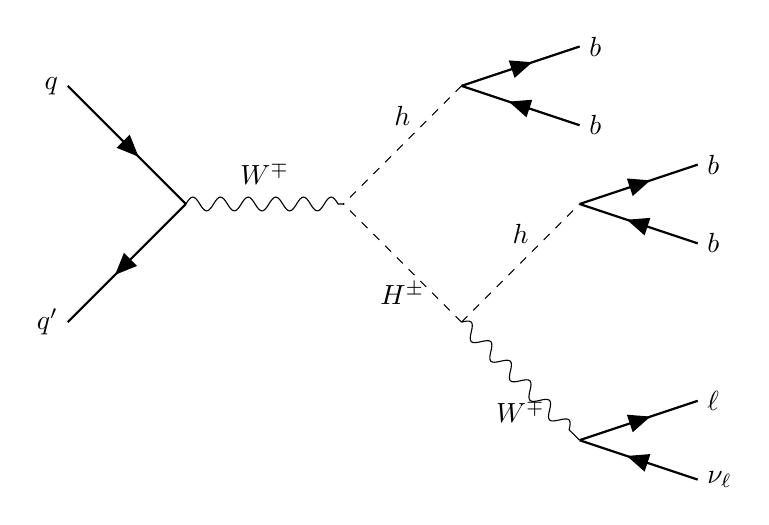
\begin{tikzpicture}[node distance=1.5cm]
    \coordinate[label=left:$q$] (q1);
    \coordinate[below=3cm of q1, label=left:$q'$] (q2);
   
    \coordinate[below =1.5cm of q1] (k1); \coordinate[right =1.5cm of k1] (v1); 
    \coordinate[right =2cm of v1] (v2); \coordinate[right =1.5cm of v2] (k2);
    
    \coordinate[above=1.5 cm of k2] (h1);
    \coordinate[below=3cm of h1] (Hc);

    \coordinate[right =1.5cm of h1] (k3); 
    \coordinate[above =0.5cm of k3, label=right:$b$] (b1); 
    \coordinate[below =0.5cm of k3, label=right:$b$] (b2);  

    \coordinate[right =1.5cm of Hc] (k4); 
    \coordinate[above =1.5cm of k4] (h2); 
    \coordinate[below =1.5cm of k4] (W); 

    \coordinate[right =1.5cm of h2] (k5); 
    \coordinate[above =0.5cm of k5, label=right:$b$] (b3); 
    \coordinate[below =0.5cm of k5, label=right:$b$] (b4);

    \coordinate[right =1.5cm of W] (k6); 
    \coordinate[above =0.5cm of k6, label=right:$\ell$] (l); 
    \coordinate[below =0.5cm of k6, label=right:$\nu_{\ell}$] (nu);

    \draw[fermion] (q1) -- (v1);
    \draw[fermion] (v1) -- (q2);
    \draw[photon] (v1) -- node[label=above:$W^{\mp}$] {} (v2);

    \draw[higgs] (h1) -- node[label=above:$h$] {} (v2);
    \draw[fermion] (h1) -- (b1);
    \draw[fermion] (b2) -- (h1);

    \draw[higgs] (Hc) -- node[label=below:$H^{\pm}$] {} (v2);
    \draw[higgs] (Hc) -- node[label=above:$h$] {} (h2);
    \draw[photon] (Hc) -- node[label=below:$W^{\mp}$] {} (W);

    \draw[fermion] (h2) -- (b3);
    \draw[fermion] (b4) -- (h2);

    \draw[fermion] (W) -- (l);
    \draw[fermion] (nu) -- (W);
\end{tikzpicture}


Used papers:

https://inis.iaea.org/collection/NCLCollectionStore/_Public/49/042/49042050.pdf?r=1&r=1
https://arxiv.org/pdf/1106.0034.pdf
https://arxiv.org/pdf/1706.07414.pdf


\end{document}
